\section{The Identity-Transformation Approach}
\label{sec:challenge}

We discuss the security requirements of privacy-preserving SSO and present the identity-transformation approach.


\subsection{Security Requirements for SSO Services}
\label{subsec:basicrequirements}

Non-anonymous SSO services \cite{OpenIDConnect,rfc6749,SAML,SAMLIdentifier,NIST2017draft} are designed to allow a \emph{legitimate} user to log into an \emph{honest} RP with her account at this RP, %correlating multiple logins,
by presenting \emph{identity tokens} issued by a \emph{trusted} IdP.
To achieve this goal, the trusted IdP issues an identity token that specifies the RP being accessed (i.e., \emph{RP designation}) and the authenticated user's identity or pseudo-identity (i.e., \emph{user identification}).
An honest RP verifies the RP's identity in the identity token before accepting it and authorizes the token holder to log in as the specified user. This prevents malicious RPs from replaying any received identity tokens to gain unauthorized access to other honest RPs as victim users.
The \emph{confidentiality} and \emph{integrity} of identity tokens are also necessary to prevent eavesdropping and tampering. Identity tokens are forwarded to the target RPs by the authenticated user and should not be revealed to any other parties. So they are usually signed by the trusted IdP and transmitted over HTTPS \cite{OpenIDConnect, rfc6749, SAML}.

The requirements for secure SSO services, i.e., RP designation, user identification, integrity, and confidentiality of identity tokens, have been extensively studied \cite{ArmandoCCCT08, SPRESSO, FettKS14, FettKS16, FettKS17}.
Any vulnerabilities that undermine these properties result in various attacks \cite{SomorovskyMSKJ12, WangCW12, ArmandoCCCPS13, ZhouE14, WangZLLYLG15, WangZLG16, YangLLZH16, MainkaMS16, MainkaMSW17, YangLCZ18, YangLS17, ShiWL19, ChenPCTKT14, ccsSunB12, DiscoveringJCS, dimvaLiM16, CaoSBKVC14, TowardsShehabM14}.
%An SSO system satisfying these four properties is secure.

\subsection{Identity Transformation}
\label{subsec:solutions}

We aim to develop a privacy-preserving SSO system that ensures security properties while preventing both IdP-based login tracing and RP-based identity linkage.
In \usso, these requirements are satisfied through \emph{transformed identities} in the identity tokens. Table \ref{tbl:notations-dilemma} lists the notations used in this paper.
The subscript $j$ and/or the superscript $i$ may be ignored if it does not cause ambiguity.

\begin{table}[htb]
\footnotesize
    \caption{The (pseudo-)identities in \usso}
    \centering
%    \begin{tabular}{|l|l|l|}
    \begin{tabular}{|p{1.0cm}|p{5.1cm}|p{1.13cm}|} \hline
    {\textbf{Notation}} & {\textbf{Description}} & {\textbf{Lifecycle}} \\ \hline
    {$ID_U$} & {The user's unique identity at the IdP.} & {Permanent} \\ \hline
    {$ID_{RP_j}$} & {The $j$-th RP's unique identity at the IdP.} & {Permanent} \\ \hline
    {$PID_{U,j}^i$} & {The user's pseudo-identity in her $i$-th login to the $j$-th RP.} & {Ephemeral} \\ \hline
    {$PID_{RP_j}^i$} & {The $j$-th RP's pseudo-identity in the user's $i$-th login to this RP.} & {Ephemeral} \\ \hline
    {$Acct_j$} & {The user's identity (or account) at the $j$-th RP.} & {Permanent} \\ \hline
    \end{tabular}
    \label{tbl:notations-dilemma}
\end{table}

In an SSO login flow, a user initiates the process by negotiating an \emph{ephemeral} pseudo-identity $PID_{RP}$  with the target RP and sending an identity-token request that encloses $PID_{RP}$ to the IdP.
After successfully authenticating the user as $ID_U$, the IdP calculates an \emph{ephemeral} $PID_U$ based on $ID_U$ and $PID_{RP}$ and issues an identity token that binds $PID_U$ and $PID_{RP}$. Upon receiving a token with a matching $PID_{RP}$, the RP calculates the user's \emph{permanent} $Acct$ and authorizes the token holder to log in.
The relationships among the permanent and ephemeral (pseudo-)identities are depicted in Figure \ref{fig:IDCorrelation}, where the \emph{red} and \emph{green} blocks represent \emph{permanent} and \emph{ephemeral} (pseudo-)identities, respectively, and the labeled arrows denote the transformations of (pseudo-)identities.

%An identity token binds the (pseudo-)identities of an authenticated user and an RP.
%Since an IdP authenticates users and then always knows the user's identity (i.e., $ID_U$),
%    to prevent the IdP-based login tracing,
%    we should not reveal the target RP's permanent identity (i.e., $ID_{RP}$) to the IdP.

For RP designation, $PID_{RP}$ should be \emph{uniquely} associated with the target RP.
For user identification, with \emph{ephemeral} $PID_{U}^i$ in each login, the designated RP should be able to derive a unique \emph{permanent} account  (i.e., $Acct$) of the user at this RP.
To prevent IdP-based login tracing, it is essential to ensure that the IdP does not obtain any information about $ID_{RP}$ from any $PID_{RP}^i$.
Thus, in a user's multiple logins to one RP,
 she should generate independent $PID_{RP}^i$s\footnote{The IdP should not be able to link multiple logins visiting a given RP, while the RP's identity is unknown to the IdP.} % the IdP-based login tracing is still effective, to correlate a user's multiple logins.
and independent $PID_U^i$s.\footnote{If $PID_U^i$ is not completely independent of each other, it implies that there is a possibility for the IdP to link multiple logins visiting a given RP.}
Finally, to prevent RP-based identity linkage,
% the IdP does not enclose $ID_U$ in identity tokens.
%a user pseudo-identity (i.e., $PID_U$) is bound instead:
%$PID_U$ is bound in identity tokens:
the RP should not obtain any information about $ID_U$ from any $PID_{U,j}$, which implies that $PID_{U,j}$ for different RPs should also be independent of each other.

\begin{figure}[bt]
  \centering
  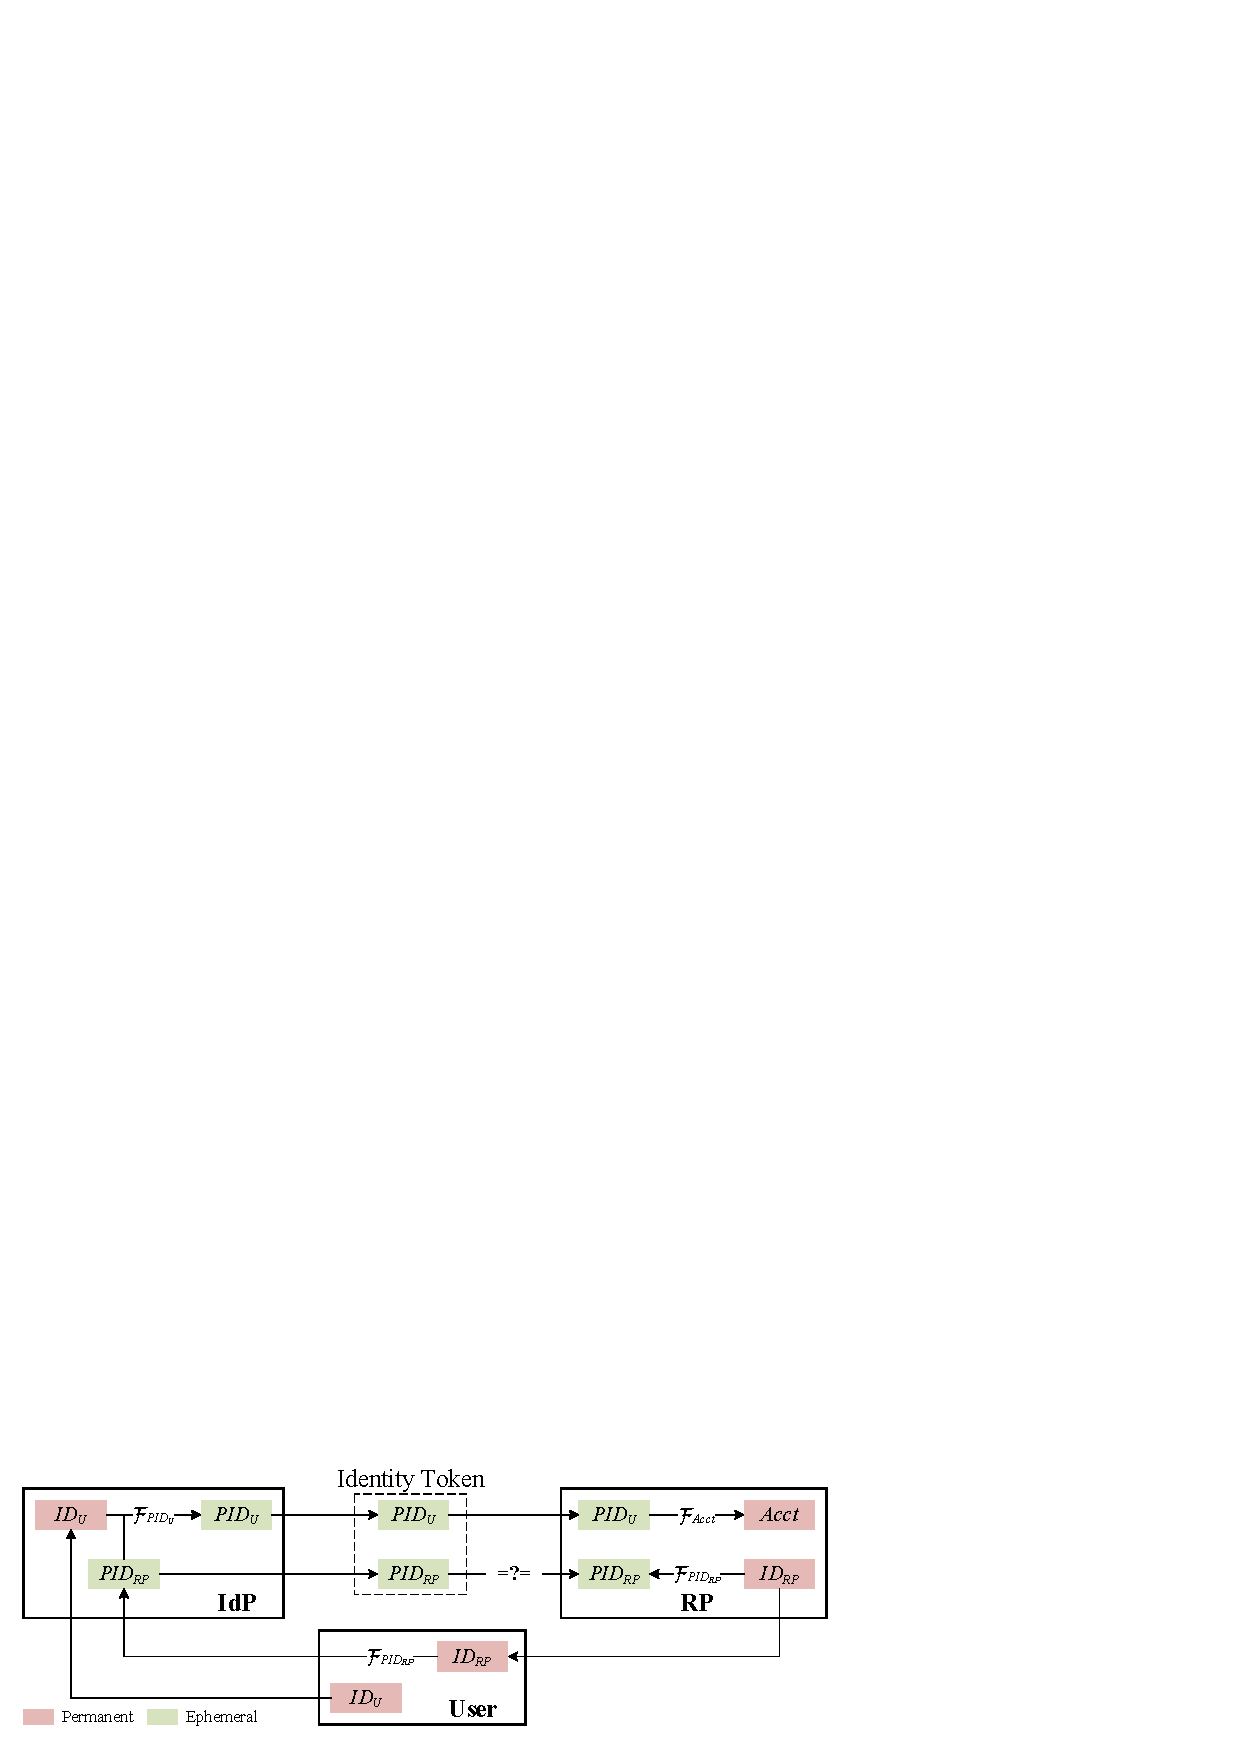
\includegraphics[width=0.99\linewidth]{fig/IDCorrelation.pdf}
  \caption{Identity transformations in \usso} %privacy-preserving SSO}
  \label{fig:IDCorrelation}
\end{figure}

We propose three identity transformations as below:
\vspace{-\topsep}\begin{itemize}
\setlength{\topsep}{0pt}
\setlength{\partopsep}{0pt}
\setlength{\itemsep}{0pt}
\setlength{\parsep}{0pt}
\setlength{\parskip}{0pt}
\item
$\mathcal{F}_{PID_{RP}}(ID_{RP}) = PID_{RP}$, calculated by the user and the RP.
In the IdP's view,
$\mathcal{F}_{PID_{RP}}()$ is a one-way function and $PID_{RP}$
is \emph{indistinguishable} from random variables.
\item
$\mathcal{F}_{PID_U}(ID_U, PID_{RP}) = PID_{U}$, calculated by the IdP.
In the target RP's view,
    $\mathcal{F}_{PID_U}()$ is a one-way function and $PID_{U}$ is \emph{indistinguishable} from random variables.
\item
$\mathcal{F}_{Acct}(PID_{U}, PID_{RP}) = Acct$, calculated by the target RP.
Given $ID_U$ and $ID_{RP}$, $Acct$ is %\emph{permanent} and
\emph{unique} to other accounts at this RP.
That is, in a user's two different logins to the RP,
 $\mathcal{F}_{Acct}(PID_{U}^i, PID_{RP}^i) = \mathcal{F}_{Acct}(PID_{U}^{i'}, PID_{RP}^{i'})$.
\end{itemize}



